%% Should be included with the command: \includestandalone[width=.30\textwidth]{tikz-diagrams/diagram}
%% Folder = tikz-diagrams ; file = tikz-diagrams/diagram.tex

\documentclass[crop,tikz,12pt]{standalone}

\usepackage{graphicx}
\usetikzlibrary{patterns}

\tikzstyle{incolore} = [
    rectangle,
    text centered,
    minimum height=0.8cm,
    text width=6.5cm
]
\tikzstyle{todo} = [
    rectangle,
    fill=gray!50,
    minimum height=0.4cm,
    anchor=west,
    draw=none
]
\tikzstyle{done} = [
    todo,
    fill=blue!65
]
\tikzstyle{hold} = [
    rectangle,
    minimum height=0.4cm,
    pattern color=blue,
    pattern=north east lines,
    anchor=west
]
\tikzstyle{doing} = [
    todo,
    fill=red!65
]

\begin{document}

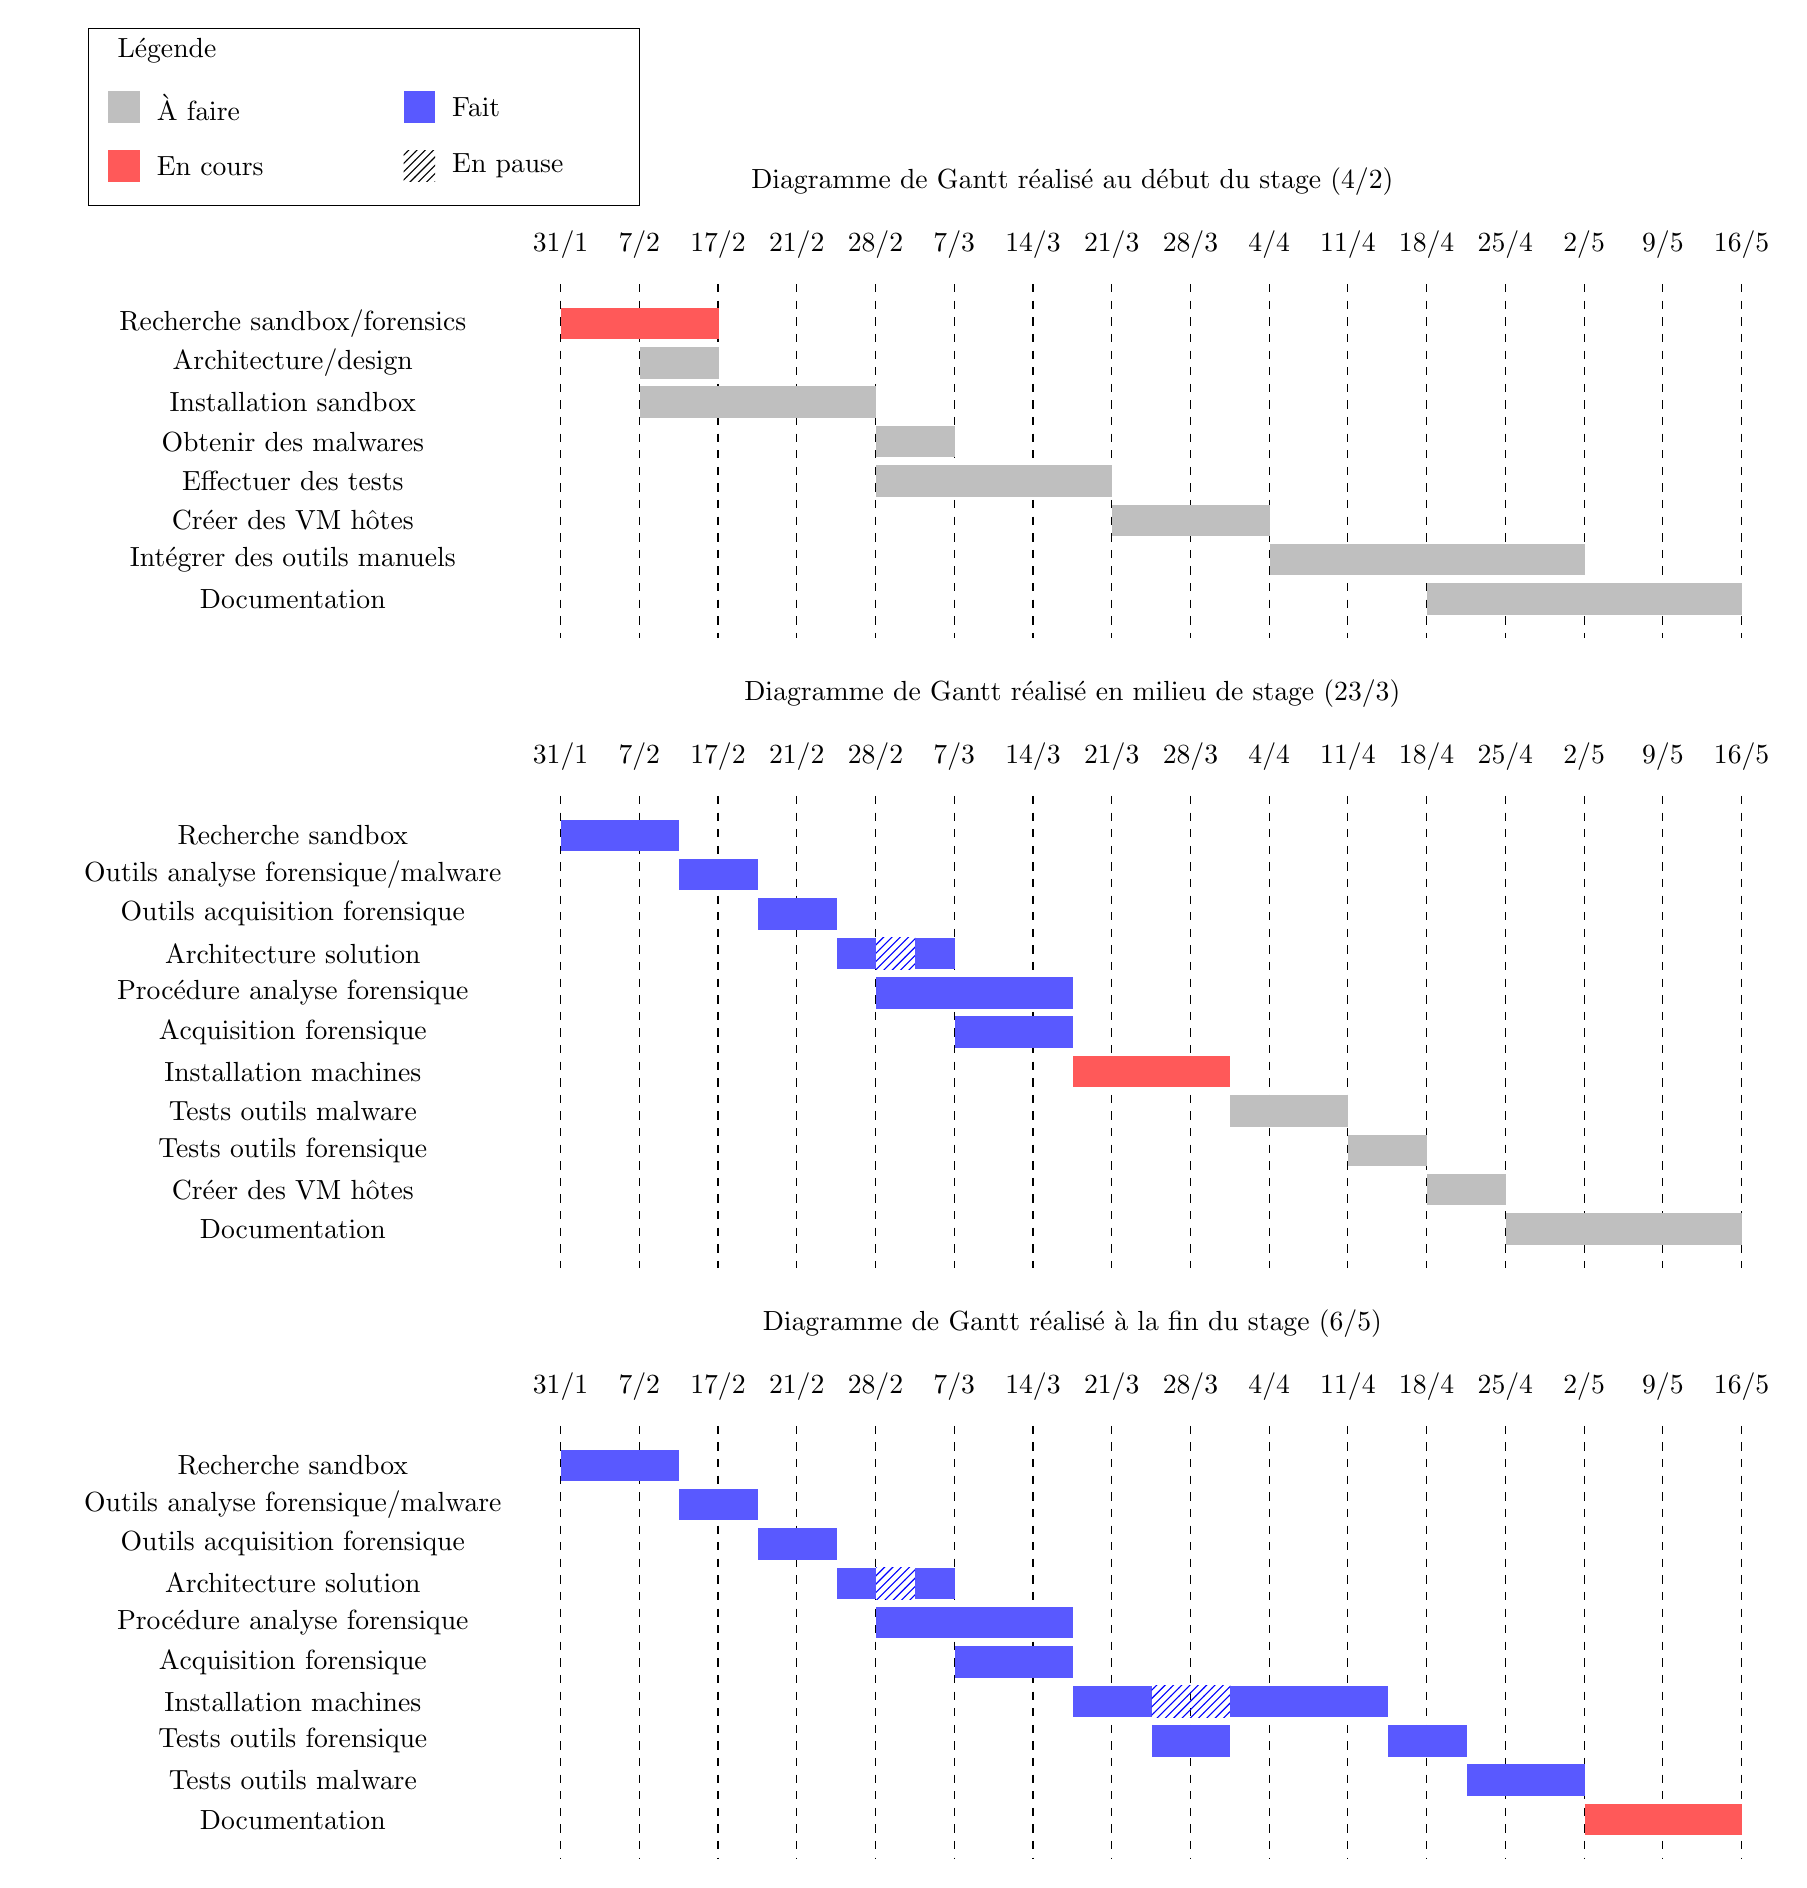
\begin{tikzpicture}

    \draw (-4,2.75) -- (3,2.75) -- (3,0.5) -- (-4,0.5) -- cycle;
    \node () [anchor=north west] at (-3.75,2.75) {Légende};

    \node () [anchor=west, fill=gray!50, minimum height=0.4cm, minimum width=0.4cm] at (-3.75,1.75) {};
    \node () [anchor=west, fill=red!65, minimum height=0.4cm, minimum width=0.4cm] at (-3.75,1.0) {};

    \node () [anchor=west] at (-3.25,1.75) {À faire};
    \node () [anchor=west] at (-3.25,1.00) {En cours};

    \node () [anchor=west, fill=blue!65, minimum height=0.4cm, minimum width=0.4cm] at (0,1.75) {};
    \node () [anchor=west, pattern=north east lines, minimum height=0.4cm, minimum width=0.4cm] at (0,1.00) {};

    \node () [anchor=west] at (0.5,1.75) {Fait};
    \node () [anchor=west] at (0.5,1.00) {En pause};

    %%%%%%%%%%%%%%%%%%%%


    \node () [] at (8.5, 0.8) {Diagramme de Gantt réalisé au début du stage (4/2)};

    \foreach \i in {1,...,16} {
        \draw[dashed] (\i+1, -0.5) -- (\i+1, -5);
    }

    \node () [] at (2,0) {31/1};
    \node () [] at (3,0) {7/2};
    \node () [] at (4,0) {17/2};
    \node () [] at (5,0) {21/2};
    \node () [] at (6,0) {28/2};

    \node () [] at (7,0)  {7/3};
    \node () [] at (8,0)  {14/3};
    \node () [] at (9,0)  {21/3};
    \node () [] at (10,0) {28/3};
    \node () [] at (11,0) {4/4};

    \node () [] at (12,0) {11/4};
    \node () [] at (13,0) {18/4};
    \node () [] at (14,0) {25/4};
    \node () [] at (15,0) {2/5};
    \node () [] at (16,0) {9/5};
    \node () [] at (17,0) {16/5};

    \node () [incolore] at (-1.4, -1.0) {Recherche sandbox/forensics};
    \node () [incolore] at (-1.4, -1.5) {Architecture/design};
    \node () [incolore] at (-1.4, -2.0) {Installation sandbox};
    \node () [incolore] at (-1.4, -2.5) {Obtenir des malwares};
    \node () [incolore] at (-1.4, -3.0) {Effectuer des tests};
    \node () [incolore] at (-1.4, -3.5) {Créer des VM hôtes};
    \node () [incolore] at (-1.4, -4.0) {Intégrer des outils manuels};
    \node () [incolore] at (-1.4, -4.5) {Documentation};

    \node () [doing, minimum width=2cm] at (2, -1.0) {};
    \node () [todo, minimum width=1cm] at (3, -1.5) {};
    \node () [todo, minimum width=3cm] at (3, -2.0) {};
    \node () [todo, minimum width=1cm] at (6, -2.5) {};
    \node () [todo, minimum width=3cm] at (6, -3.0) {};
    \node () [todo, minimum width=2cm] at (9, -3.5) {};
    \node () [todo, minimum width=4cm] at (11,-4.0) {};
    \node () [todo, minimum width=4cm] at (13,-4.5) {};


    %%%%%%%%%%%%%%%%%%%%


    \node () [] at (8.5, 0.8-6.5) {Diagramme de Gantt réalisé en milieu de stage (23/3)};

    \foreach \i in {1,...,16} {
        \draw[dashed] (\i+1, -0.5-6.5) -- (\i+1, -6.5-6.5);
    }

    \node () [] at (2,0-6.5) {31/1};
    \node () [] at (3,0-6.5) {7/2};
    \node () [] at (4,0-6.5) {17/2};
    \node () [] at (5,0-6.5) {21/2};
    \node () [] at (6,0-6.5) {28/2};

    \node () [] at (7,0-6.5)  {7/3};
    \node () [] at (8,0-6.5)  {14/3};
    \node () [] at (9,0-6.5)  {21/3};
    \node () [] at (10,0-6.5) {28/3};
    \node () [] at (11,0-6.5) {4/4};

    \node () [] at (12,0-6.5) {11/4};
    \node () [] at (13,0-6.5) {18/4};
    \node () [] at (14,0-6.5) {25/4};
    \node () [] at (15,0-6.5) {2/5};
    \node () [] at (16,0-6.5) {9/5};
    \node () [] at (17,0-6.5) {16/5};

    \node () [incolore] at (-1.4, -1.0-6.5) {Recherche sandbox};
    \node () [incolore] at (-1.4, -1.5-6.5) {Outils analyse forensique/malware};
    \node () [incolore] at (-1.4, -2.0-6.5) {Outils acquisition forensique};
    \node () [incolore] at (-1.4, -2.5-6.5) {Architecture solution};
    \node () [incolore] at (-1.4, -3.0-6.5) {Procédure analyse forensique};
    \node () [incolore] at (-1.4, -3.5-6.5) {Acquisition forensique};
    \node () [incolore] at (-1.4, -4.0-6.5) {Installation machines};
    \node () [incolore] at (-1.4, -4.5-6.5) {Tests outils malware};
    \node () [incolore] at (-1.4, -5.0-6.5) {Tests outils forensique};
    \node () [incolore] at (-1.4, -5.5-6.5) {Créer des VM hôtes};
    \node () [incolore] at (-1.4, -6.0-6.5) {Documentation};

    \node () [done, minimum width=1.5cm] at (2,   -1.0-6.5) {};
    \node () [done, minimum width=1.0cm] at (3.5, -1.5-6.5) {};
    \node () [done, minimum width=1.0cm] at (4.5, -2.0-6.5) {};

    \node () [done, minimum width=0.5cm] at (5.5, -2.5-6.5) {};
    \node () [hold, minimum width=0.5cm] at (6.0, -2.5-6.5) {};
    \node () [done, minimum width=0.5cm] at (6.5, -2.5-6.5) {};

    \node () [done, minimum width=2.5cm] at (6.0, -3.0-6.5) {};
    % \node () [done, minimum width=0.5cm] at (6.5, -3.0) {};
    % \node () [done, minimum width=0.5cm] at (7.0, -3.0) {};
    % \node () [hold, minimum width=0.5cm] at (7.5, -3.0) {};
    % \node () [done, minimum width=0.5cm] at (8.0, -3.0) {};

    \node () [done, minimum width=1.5cm] at (7.0, -3.5-6.5) {};
    \node () [doing, minimum width=2.0cm] at (8.5,-4.0-6.5) {};

    \node () [todo, minimum width=1.5cm] at (10.5,-4.5-6.5) {};
    \node () [todo, minimum width=1.0cm] at (12.0,-5.0-6.5) {};
    \node () [todo, minimum width=1.0cm] at (13,-5.5-6.5) {};
    \node () [todo, minimum width=3.0cm] at (14,-6.0-6.5) {};


    %%%%%%%%%%%%%%%%%%%%


    \node () [] at (8.5, 0.8-14.5) {Diagramme de Gantt réalisé à la fin du stage (6/5)};

    \foreach \i in {1,...,16} {
        \draw[dashed] (\i+1, -0.5-14.5) -- (\i+1, -6.0-14.5);
    }

    \node () [] at (2,0-14.5) {31/1};
    \node () [] at (3,0-14.5) {7/2};
    \node () [] at (4,0-14.5) {17/2};
    \node () [] at (5,0-14.5) {21/2};
    \node () [] at (6,0-14.5) {28/2};

    \node () [] at (7,0-14.5)  {7/3};
    \node () [] at (8,0-14.5)  {14/3};
    \node () [] at (9,0-14.5)  {21/3};
    \node () [] at (10,0-14.5) {28/3};
    \node () [] at (11,0-14.5) {4/4};

    \node () [] at (12,0-14.5) {11/4};
    \node () [] at (13,0-14.5) {18/4};
    \node () [] at (14,0-14.5) {25/4};
    \node () [] at (15,0-14.5) {2/5};
    \node () [] at (16,0-14.5) {9/5};
    \node () [] at (17,0-14.5) {16/5};

    \node () [incolore] at (-1.4, -1.0-14.5) {Recherche sandbox};
    \node () [incolore] at (-1.4, -1.5-14.5) {Outils analyse forensique/malware};
    \node () [incolore] at (-1.4, -2.0-14.5) {Outils acquisition forensique};
    \node () [incolore] at (-1.4, -2.5-14.5) {Architecture solution};
    \node () [incolore] at (-1.4, -3.0-14.5) {Procédure analyse forensique};
    \node () [incolore] at (-1.4, -3.5-14.5) {Acquisition forensique};
    \node () [incolore] at (-1.4, -4.0-14.5) {Installation machines};
    \node () [incolore] at (-1.4, -4.5-14.5) {Tests outils forensique};
    \node () [incolore] at (-1.4, -5.0-14.5) {Tests outils malware};
    \node () [incolore] at (-1.4, -5.5-14.5) {Documentation};

    \node () [done, minimum width=1.5cm] at (2,   -1.0-14.5) {};
    \node () [done, minimum width=1.0cm] at (3.5, -1.5-14.5) {};
    \node () [done, minimum width=1.0cm] at (4.5, -2.0-14.5) {};

    \node () [done, minimum width=0.5cm] at (5.5, -2.5-14.5) {};
    \node () [hold, minimum width=0.5cm] at (6.0, -2.5-14.5) {};
    \node () [done, minimum width=0.5cm] at (6.5, -2.5-14.5) {};

    \node () [done, minimum width=2.5cm] at (6.0, -3.0-14.5) {};
    \node () [done, minimum width=1.5cm] at (7.0, -3.5-14.5) {};

    % installation
    \node () [done, minimum width=1.0cm] at (8.5,-4.0-14.5) {};
    \node () [hold, minimum width=1.0cm] at (9.5,-4.0-14.5) {};
    \node () [done, minimum width=2.0cm] at (10.5,-4.0-14.5) {};

    % forensique
    \node () [done, minimum width=1.0cm] at (9.5,-4.5-14.5) {};
    \node () [done, minimum width=1.0cm] at (12.5,-4.5-14.5) {};

    % analyse malware
    \node () [done, minimum width=1.5cm] at (13.5,-5.0-14.5) {};

    % documentation
    \node () [doing, minimum width=2.0cm] at (15,-5.5-14.5) {};

\end{tikzpicture}

\end{document}
